% Exam Template for UMTYMP and Math Department courses
%
% Using Philip Hirschhorn's exam.cls: http://www-math.mit.edu/~psh/#ExamCls
%
% run pdflatex on a finished exam at least three times to do the grading table on front page.
%
%%%%%%%%%%%%%%%%%%%%%%%%%%%%%%%%%%%%%%%%%%%%%%%%%%%%%%%%%%%%%%%%%%%%%%%%%%%%%%%%%%%%%%%%%%%%%%

% These lines can probably stay unchanged, although you can remove the last
% two packages if you're not making pictures with tikz.
\documentclass[11pt]{exam}
\RequirePackage{amssymb, amsfonts, amsmath, latexsym, verbatim, xspace, setspace}
\RequirePackage{tikz, pgflibraryplotmarks}

% By default LaTeX uses large margins.  This doesn't work well on exams; problems
% end up in the "middle" of the page, reducing the amount of space for students
% to work on them.
\usepackage[margin=1in]{geometry}
%\usepackage{tkz-euclide}
\usepackage{multicol}
\usepackage{graphicx}
\usepackage{tikz,pgfplots}
\usepackage{listings}
\usepackage{pdfpages}
\usepackage{minitoc} %% Required
\usepackage{tabularx}

% Here's where you edit the Class, Exam, Date, etc.
\newcommand{\class}{Calculus I}
\newcommand{\term}{Fall 2020}
\newcommand{\examnum}{Lab 5}
\newcommand{\examdate}{August 20, 2020}

% For an exam, single spacing is most appropriate
\singlespacing
% \onehalfspacing
% \doublespacing

% For an exam, we generally want to turn off paragraph indentation
\parindent 0ex

\begin{document} 
	
	% These commands set up the running header on the top of the exam pages
	\pagestyle{head}
	\firstpageheader{}{}{}
	\runningheader{\class}{\examnum\ - Page \thepage\ of \numpages}{\term}
	\runningheadrule
	
	\begin{flushright}
		\begin{tabular}{p{2.8in} r l}
			\textbf{\class} & \textbf{Name (Print):} & \makebox[2in]{\hrulefill}\\
			\textbf{\term} &&\\
			\textbf{\examnum} &&\\
			%\textbf{\examdate} &&\\
			%\textbf{Due Date: \duedate}
			%\textbf{Time Limit: \timelimit} & Teaching Assistant & \makebox[2in]{\hrulefill}
		\end{tabular}\\
	\end{flushright}
	
Show all your work, cite your sources, and type your answers for full credit.\\

Materials needed: none
	
	\rule[1ex]{\textwidth}{.1pt}
	
	\setlength{\columnsep}{0.5 in}
	
	\begin{questions}
		
		\addpoints
		
		\question[0] (In Class Activity) draw a function and the derivative of that function on the same graph.  Draw the derivative of the derivative function (this is called the second derivative) on that same graph as well.  Label each I, II, III and provide the answers under a piece of paper taped on the white board
		
		\question[5] Using what you've learned from Calculus lecture, find a formula for
		\[
		\frac{d}{d x} \left( \frac{f(x)}{g(x)h(x)} \right)
		\]
		
			\question[5] Using what you've learned from Calculus lecture, find a formula for
		\[
		\frac{d}{d x} \Big( f(x)g(x)h(x) \Big)
		\]
		
		\question[5] Find the three tangent lines to the curve $f(x)=(x+2)(x-3)(x+4)$ that go through the point $(4,-7)$.
		
		\newpage
		
		\question[10] Let $f$ and $g$ be defined by the graph below.
		
		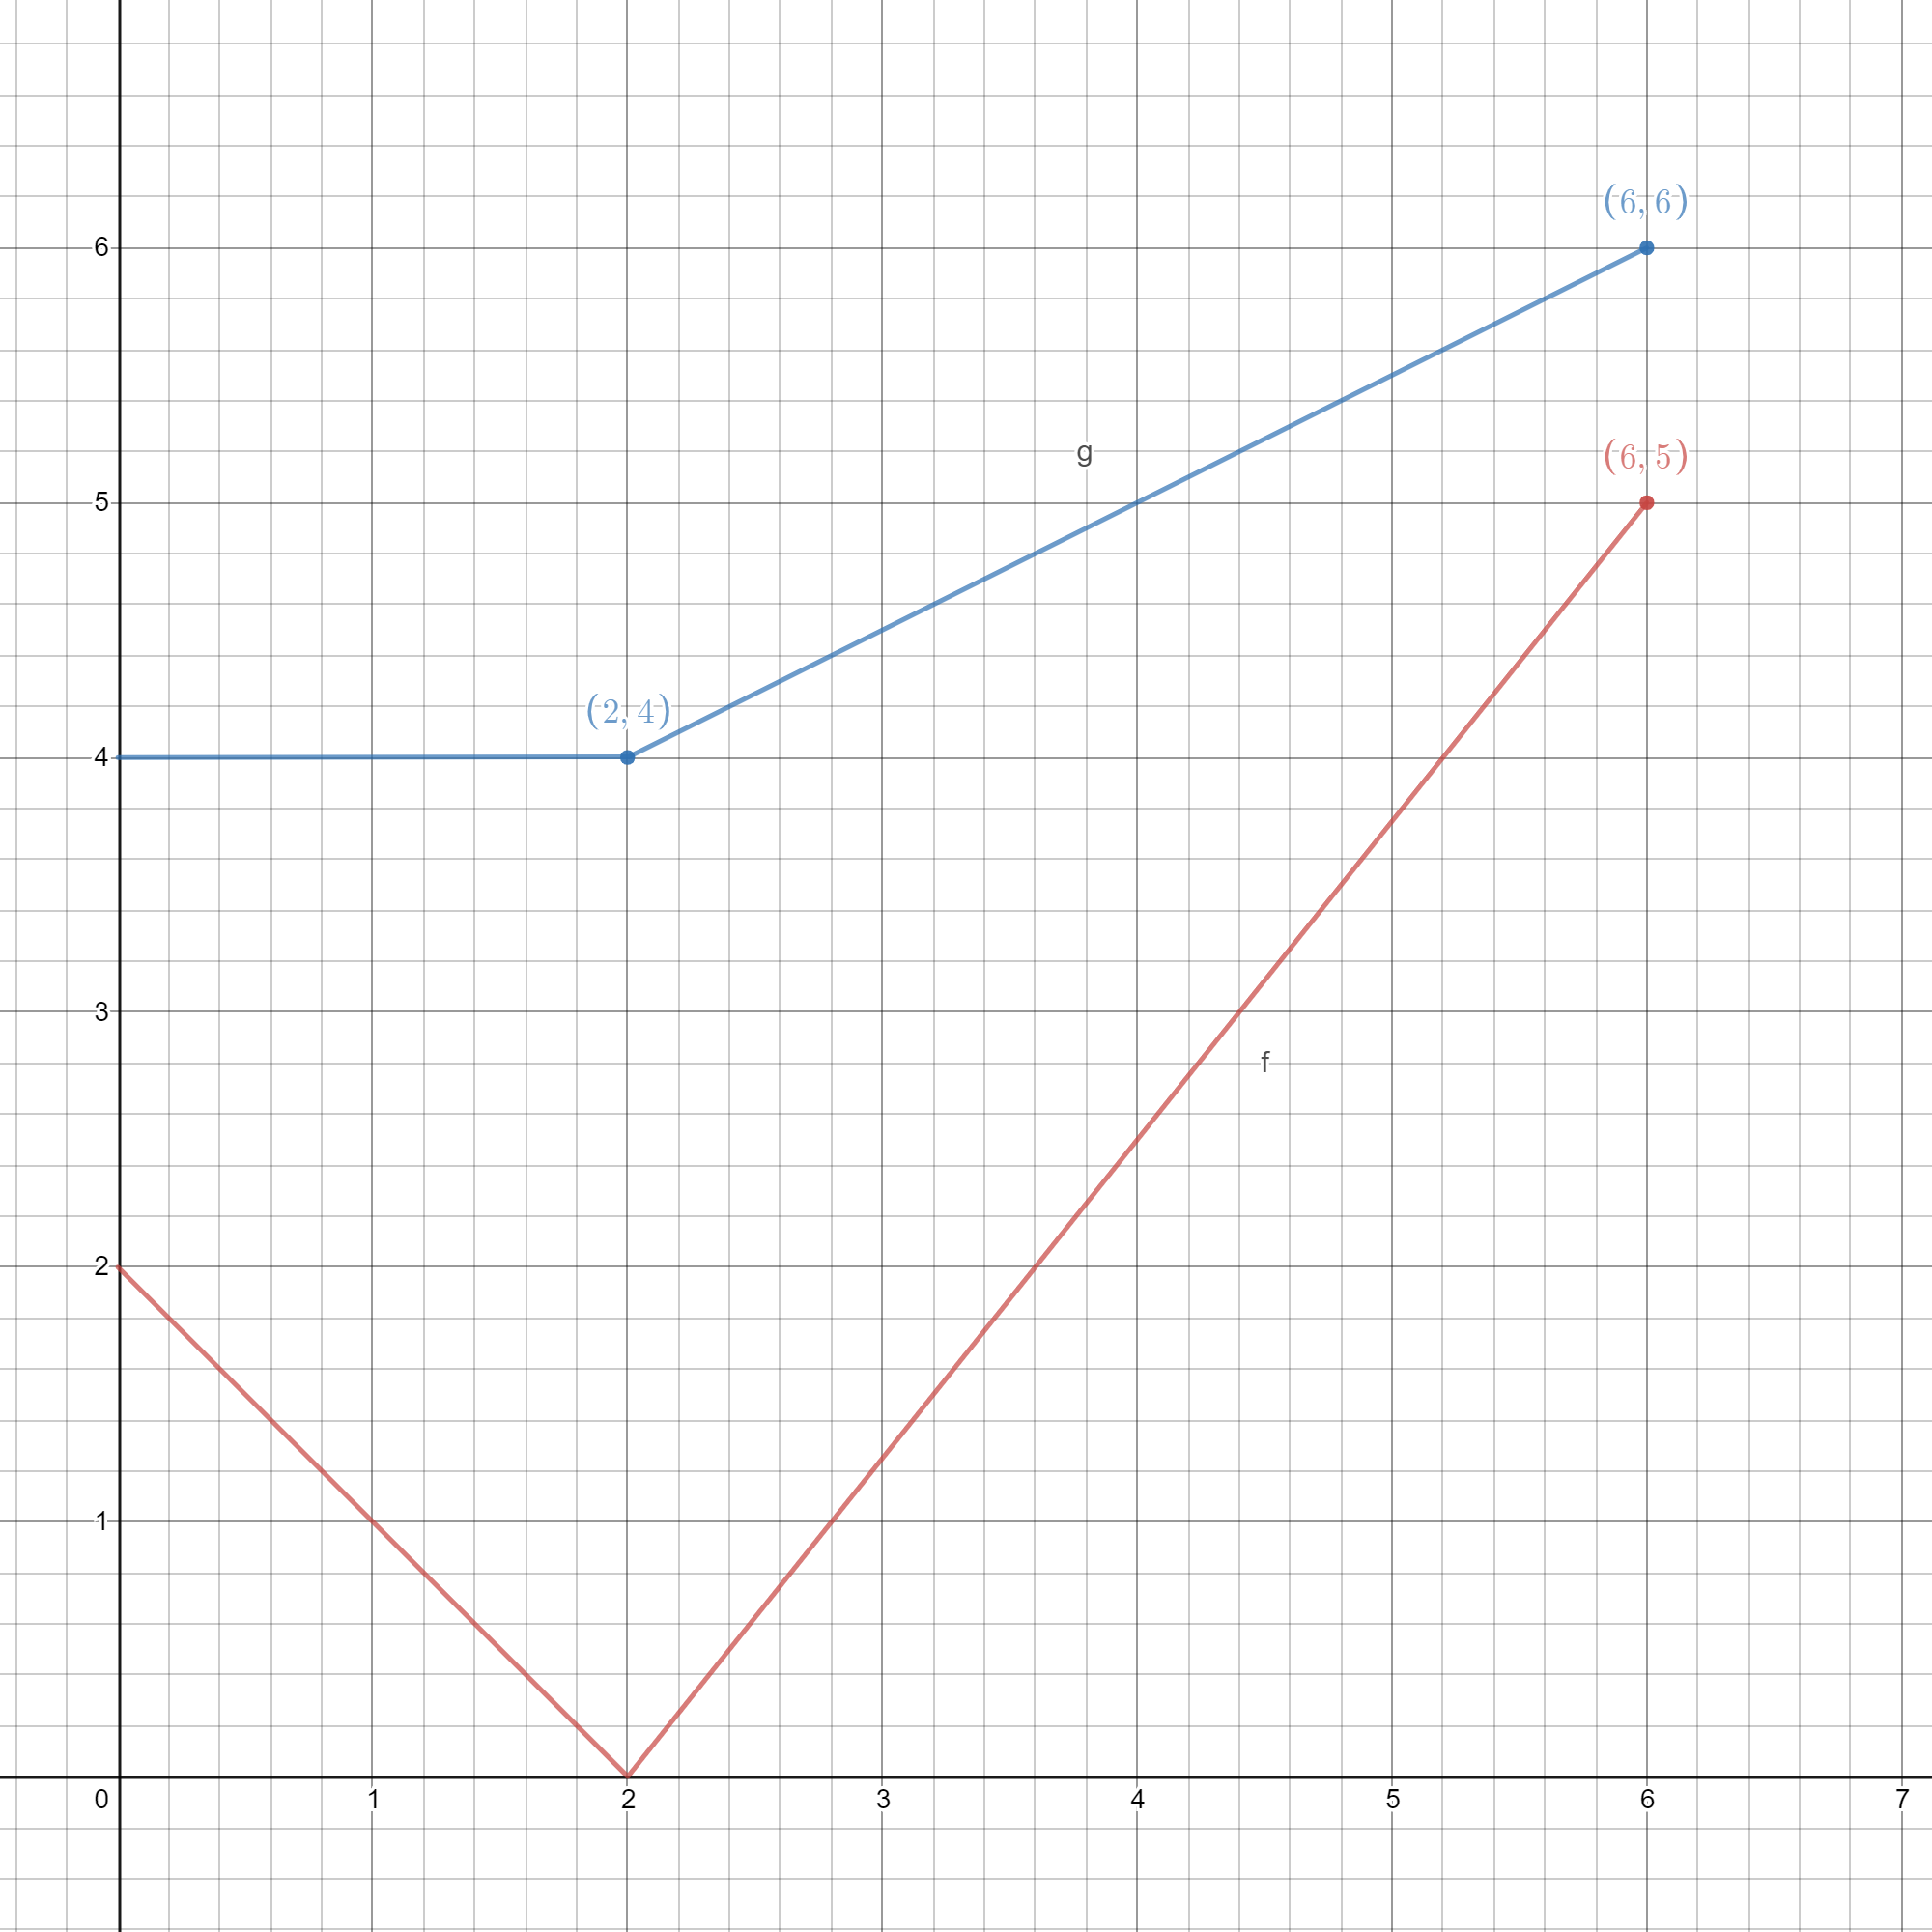
\includegraphics[width = 5 in]{images/desmos-lab-5.png}
		
		Let
		\[
		r(x) = f(g(x)) \hspace{.5 in} s(x) = g(f(x)), \hspace{.5 in} t(x) = f(x)g(x), \hspace{.5 in} u(x) = \frac{f(x)}{g(x)}
		\]
		Compute the following:
		\begin{multicols}{2}
			\begin{parts}
			\part $r' (1)$ 
			\part $r' (4) $
			\part $s'(1) $
			\part $s' (4)$ 
			\part $t' (1)$
			\part $t' (4)$
			\part $u'(1)$
			\part $u' (4)$
			\end{parts}
		\end{multicols}
		
	\end{questions}
	
\end{document}
